\documentclass[12pt]{article}
%Gumm{\color{blue}i}|065|=)
\usepackage{amsmath, amsfonts, amssymb}
\usepackage[margin=0.5in]{geometry}
\usepackage{xcolor}
\usepackage{graphicx}
\usepackage{amsmath}
\usepackage{hyperref}

\newcommand{\off}[1]{}
\DeclareMathSizes{20}{30}{20}{18}
\usepackage{tikz}


\title{Reading: Tilings with Triangles}
\date{}
\begin{document}

\sffamily

\maketitle

\noindent We just want to understand a little bit better the article in ``Communications in Theoretical Physics" \textbf{The Isoperimetric Problem for Pinwheel Tilings}.   
\begin{itemize}
\item what was the isoperimetric problem?
\item what kind of tilings can we make with these shapes 
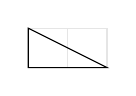
\begin{tikzpicture}[scale=0.5]
\draw[black!10!white] (0,0)--(1,0)--(2,0)--(2,1)--(1,1)--(0,1)--cycle;
\draw[black!10!white] (1,0)--(1,1);
\draw(0,0)--(2,0)--(0,1)--cycle;
\end{tikzpicture} and
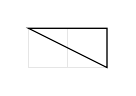
\begin{tikzpicture}[scale=0.5]
\draw[black!10!white] (0,0)--(1,0)--(2,0)--(2,1)--(1,1)--(0,1)--cycle;
\draw[black!10!white] (1,0)--(1,1);
\draw(0,1)--(2,0)--(2,1)--cycle;
\end{tikzpicture} .  These are parts of $2 \times 1$ rectangle.
\item What is Charles Radin calling the ``isoperimetric problem" here\dots how to these shapes lead to shapes that are area-minimizing or circumference-minimizing or just plain, close to circular. 
\end{itemize}
First of all, let's draw a single tile with the points. \\ \\
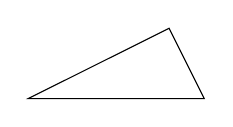
\begin{tikzpicture}
\draw(0,0)--(2.236,0)--(1.789,0.894)--cycle;
\end{tikzpicture} \\ 
As a computer programmer, we are tempted to accept the first solution that looks like it works.  Orthogonal to this are other solutions -- other computer program implementations -- which produce the same image.  What if we change the problem?  For now, since there is only one example, let's take the first solution that works. \\ \\
This is already a geometry problem, since I had to draw all three points.  Let's try to assign a length to each side, and maybe coordinates.  If we only do Euclidean Geometry, there are no coordinates, we don't get anything like coordinates until Descartes and then it's Analytic Geometry. \\
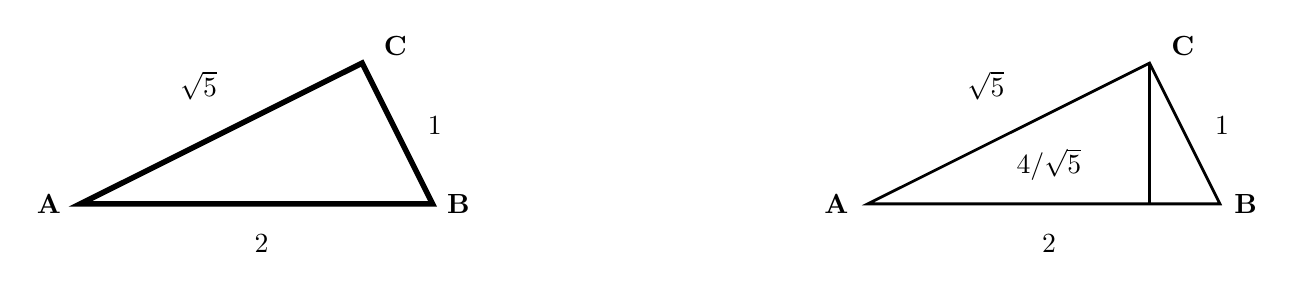
\begin{tikzpicture}[scale=2]
% decimals questionable
\begin{scope}
\draw[line width=2](0,0)--(2.236,0)--(1.789,0.894)--cycle;
\node at (1.15,-0.25) {$2$};
\node at (2.25, 0.5) {$1$};
\node at (0.75, 0.75) {$\sqrt{5}$};
\node at (-0.2,0) {\textbf{A}};
\node at (2.4,0) {\textbf{B}};
\node at (2,1) {\textbf{C}};
\end{scope}
\begin{scope}[xshift=5cm]
\draw[line width=1](0,0)--(2.236,0)--(1.789,0.894)--cycle;
\node at (1.15,-0.25) {$2$};
\node at (1.15, 0.25) {$4/\sqrt{5}$};
\node at (2.25, 0.5) {$1$};
\node at (0.75, 0.75) {$\sqrt{5}$};
\node at (-0.2,0) {\textbf{A}};
\node at (2.4,0) {\textbf{B}};
\node at (2,1) {\textbf{C}};
\draw[line width=1] (1.789,0)--(1.789,0.894);
\end{scope}
\end{tikzpicture} \\
Our computer program has chosen to use coordinates.  Standard high school question is to find the height of the \textbf{altitude} of the top point, \textbf{B}.   \\\\
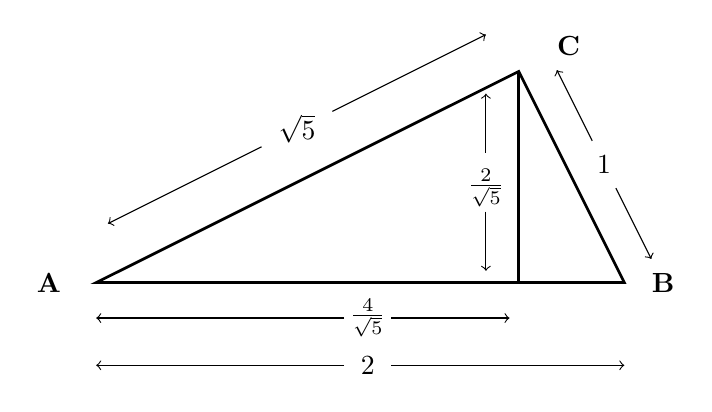
\begin{tikzpicture}[scale=3]
% decimals questionable
\draw[line width=1](0,0)--(2.236,0)--(1.789,0.894)--cycle;
\node at (1.15,-0.35) {$2$};
\node at (1.15,-0.15) {$\frac{4}{\sqrt{5}}$};
\node at (1.65, 0.4) {$\frac{2}{\sqrt{5}}$};
\node at (2.15, 0.5) {$1$};
\node at (0.85, 0.65) {$\sqrt{5}$};
\draw[->] (0.85 + 0.3*0.5, 0.65 + 0.15*0.5)--(0.85 + 1.6*0.5,0.65 + 0.8*0.5);
\draw[->] (0.85 - 0.3*0.5, 0.65 - 0.15*0.5)--(0.85 - 1.6*0.5,0.65 - 0.8*0.5);
\node at (-0.2,0) {\textbf{A}};
\node at (2.4,0) {\textbf{B}};
\node at (2,1) {\textbf{C}};
\draw[line width=1] (1.789,0)--(1.789,0.894);
\draw[->] (1.25, -0.35)--(2.236,-0.35);
\draw[->] (1.05, -0.35)--(0,    -0.35);
\draw[->] (1.25, -0.15)--(1.75, -0.15);
\draw[->] (1.05, -0.15)--(0,    -0.15);
\draw[->] (1.65,0.3)--(1.65,0.05);
\draw[->] (1.65,0.55)--(1.65,0.8);
\draw[->] (2.15 + 1*0.05 ,0.5  - 2*0.05)--(2.15 + 1*0.2,0.5 - 2*0.2);
\draw[->] (2.15 - 1*0.05 ,0.5  + 2*0.05)--(2.15 - 1*0.2,0.5 + 2*0.2);
\end{tikzpicture} \\ 
Having drawn as many arrows as we can, let's try to find the theorem for this triangles.  

\newpage

\noindent If we draw more and more altitudes of the right triangles we can find a perfect dissection into similar figures.  It might be good to ask if such a decomposition exists for $3 \times 1$ rectangles (and right triangles). \\ \\ 
Radin and Sadun's procedure is to iterate this decomposition over and over and we can find different shapes.  We will be looking for shapes that are close to a circle.

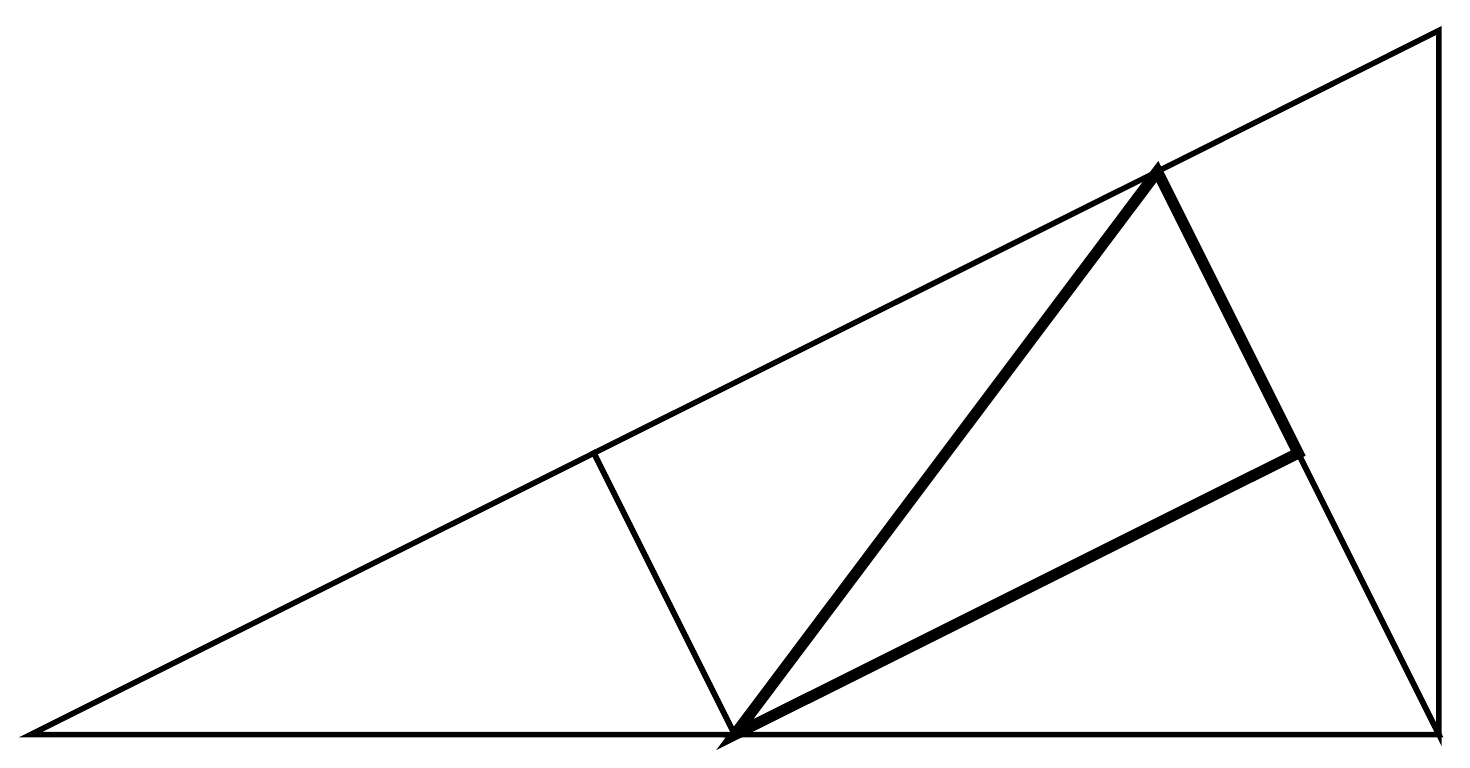
\begin{tikzpicture}[scale=4]
\draw[line width=2](0,0)--(2.236,0)--(1.789,0.894)--cycle;
\draw[line width=2](0 + 2*1.789 - 2*0 ,0 + 2*0.894 - 2*0 )--(2.236,0)--(1.789,0.894)--cycle;
\draw[line width=4](2.236,0)--(2.236+1.789, 0+0.894)--(2.236 + 1.789 - 2.236 + 1.789 , 0 + 0.894 + 0.894 - 0 )--cycle;
\draw[line width=2] (1*2.236,0)--(2*2.236,0)--(2.236+1.789, 0+0.894)--cycle;
\draw[line width=2] (2*2.236,0)--(2*2.236,2.236)--(2*1.789 , 2*0.894)--cycle;
\end{tikzpicture} \\ \\
Three decimal places leads to some interesting arithmetic problems. \\
$2( 2.236 , 0 )+ ( 0 , 2.236 ) = 2( 1.789, 0.894) + ( 2\times(2.236-1.789) , 2.236) \approx \sqrt{5}(2,1) $ \\
And if we replace these appromations with $\sqrt{1^2 + 2^2} = \sqrt{5}$ we should be able to find an exact answer. \\
$ 2( \sqrt{5},0) + (0,\sqrt{5}) = \sqrt{5}(2,1) $ \\
If we draw with line segments instead of cycles these are less artifacts. These errors seem to have resolved already at the $10^{-3}$ scale. The published article uses the cycles.  \\
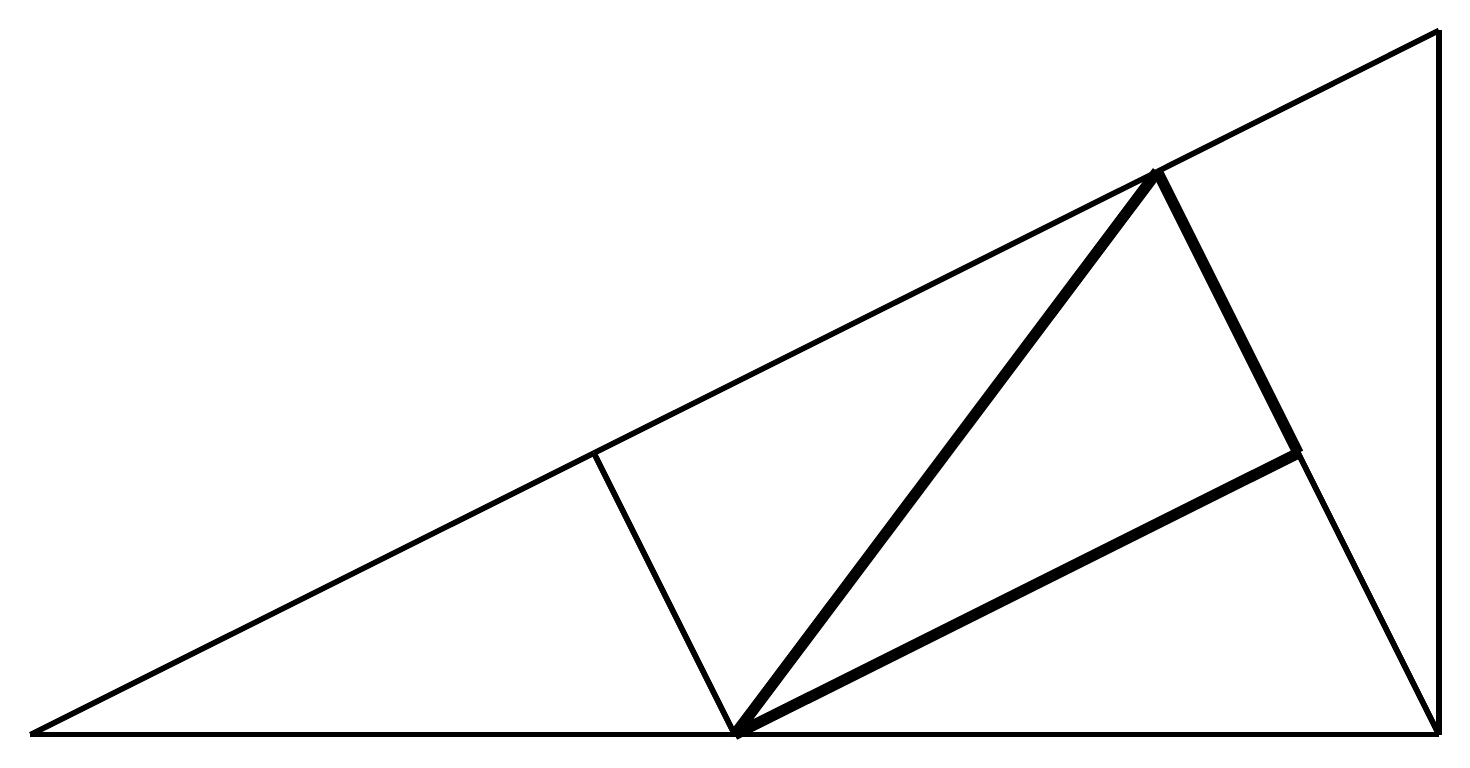
\begin{tikzpicture}[scale=4]
\draw[line width=2](0,0)--(2.236,0);
\draw[line width=2](2.236,0)--(1.789,0.894);
\draw[line width=2](1.789,0.894)--(0,0);
%
\draw[line width=2](0 + 2*1.789 - 2*0 ,0 + 2*0.894 - 2*0 )--(2.236,0);
\draw[line width=2](2.236,0)--(1.789,0.894);
\draw[line width=2](1.789,0.894)--(0 + 2*1.789 - 2*0 ,0 + 2*0.894 - 2*0 );
%
\draw[line width=4](2.236,0)--(2.236+1.789, 0+0.894);
\draw[line width=4](2.236+1.789, 0+0.894)--(2.236 + 1.789 - 2.236 + 1.789 , 0 + 0.894 + 0.894 - 0 );
\draw[line width=4](2.236 + 1.789 - 2.236 + 1.789 , 0 + 0.894 + 0.894 - 0 )--(2.236,0);
%
\draw[line width=2] (1*2.236,0)--(2*2.236,0);
\draw[line width=2] (2*2.236,0)--(2.236+1.789, 0+0.894);
\draw[line width=2] (2.236+1.789, 0+0.894)--(1*2.236,0);
%
\draw[line width=2] (2*2.236,0)--(2*2.236,2.236);
\draw[line width=2] (2*2.236,2.236)--(2*1.789 , 2*0.894);
\draw[line width=2] (2*1.789 , 2*0.894)--(2*2.236,0);
\end{tikzpicture} 

\newpage \noindent What were the two main ideas of the paper? \\ \\
\textbf{Thm \#1} Given $\epsilon > 0$ there is a distance $\mathbb{R}$ such that for any disc $C$ and radius $r < R$ there is a region $D$ whose boundary follows the edges of triangles in a tiling, that approximates $C$ in the sense that
$$ |(\text{perimeter of }D) - 2\pi r| < \epsilon r \text{ and }(\text{area of }C\backslash D) + (\text{area of }D\backslash C) < \epsilon r^2 $$
In particular, $(\text{area of }D)/(\text{perimeter of }D)^2 > (4\pi)^{-1} - \epsilon $. \\ \\
Let's check that for a perfect circle, the radio of the circumference and the diameter  $ \frac{A}{D} = \frac{\pi r^2}{(\pi d)^2} = \frac{1}{4\pi} $. \\ This constant is the same for all circles. \footnote{Constants, $\mathbb{R}$. Construction of the real numbers.}\\ \\ 
So given large amounts of triangles, we can approximate a circular region, and the main tool we have to evaluate properties of regions that are close-to-circular is {measure theory}. \\ \\
The edges of a triangles form a \textbf{metric space}.  The other theorem is to check that the distance between two lines is close a straight line. \\ \\
\textbf{Thm \#2} Given any $\epsilon > 0$ there exists $R > 0$ such that for any two points $P, Q$ on the boundaries of triangles $||P-Q|| > R$ there is a path $h$ along the boundaries of these triangles, connecting $P$ to $Q$ with length $|h|$ satisfying 
$$ \frac{|h| - ||P-Q||}{||P - Q||} < \epsilon  $$
How do we measure the closeness of two paths (``approximate lines")? how did our tiling generate metric spaces that are approximate to a regions (``approximate circles")?  How do we measure the closeness of area or perimeter?  The measure theory section of a Real Analysis textbook could give us bounds or parameters to play with. \\ \\
Looking at the bibliography, this article was published in Communications in Mathematical Physics in 1996, and this discussion was in Annals of Mathematics in 1994.  Local-to-global princples, crystallography and group theory (even though are tilings are chaotic), percolation theory and ergodic theory.  The chaotic and yet symmetric nature of these elementary geometric shapes. \\ \\
I could not find another deomposition of the $2 \times 1$ triangle into five copies of similiar triangles $\frac{1}{5}(2 \otimes 1)$.  Also, the points of these complicated triangle arrangements all lie in the same number fields $\mathbb{Q}(\sqrt{5})$ or $\mathbb{Z}[\sqrt{5}]$ if we define a single building block. \\ \\
The books are actually old and computers and computer graphics have improved between 1980 and 2020. Here, for example, I don't think we can find tilings exactly the same.  They are close to these same region.  What does that mean that $\mu(C \backslash D) < \epsilon$, what are we measuring that we call ``area"? \\ \\
$\theta = \tan^{-1} \frac{1}{2}$.  This angle is not special either.  These authors have showed a sample of the very special shapes (or metric space, etc.) that can occur.  The objects or classes of objects being constructed require more reading and discussion.

\vfill



\begin{thebibliography}{}

\item Charles Radin, Lorenzo Sadun.  \textbf{The isoperimetric problem for pinwheel tilings}. Communications in Mathematical Physics 177 p. 255-263 (1996).
\item Charles Radin \textbf{Miles of Tiles} (Student Mathematical Library \#1) American Mathematcal Society, 1999.
\item 
Michael Baake, Dirk Frettlöh, Uwe Grimm \textbf{A radial analogue of Poisson's summation formula with applications to powder diffraction and pinwheel patterns} \texttt{arXiv:math/0610408}
\item Michael F. Whittaker \textbf{C* algebras of tilings with infinite rotational symmetry} \texttt{arXiv:1010.1991}
\item Michael Baake, Uwe Grimm. \textbf{Mathematical diffraction of aperiodic structures} \texttt{arXiv:1205.3633}
\end{thebibliography} 

\end{document}